\scanpage{39}\mspage{38}
% @continuation
également stable par passage à une sous-contrée. Enfin, si $\unsure{C|\mathcal C}$ est finitiste, $\unsure{C'|C}$ aussi\unsure{?|:|.}
% @disj

\uuline{\deleted{Figures} disjointes} On dit que deux figures sont disjointes si elles sont compatibles, et si leur intersection est vide (\unsure{pas|que} de multistrates communes).
% @warn
% slanted
\margin{\uline{attention} Pour que deux figures ($=$ élémentaires) soient disjointes, il \unsure{est} \uuline{néc}, mais \deleted{\unsure{pas}} \inserted{néc} \unsure{suffis|suffisant} que leurs ombres soient disjointes (\unsure{c.à.d.} : \unsure{cp paires|cp pour} \unsure{simplifient} pour deux lieux !)}
% @warn2
\margin{\unsure{si|Si} \deleted{\unsure{de}} elles sont compatibles, \deleted{\unsure{et}} et \unsure{?}\par
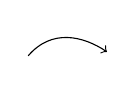
\begin{tikzpicture}[x=1cm,y=1cm]\draw[->] (0,0) .. controls (.3,.35) and (.7,.25) .. (1,.05);\end{tikzpicture}}
% @objects
On dit que \inserted{\uline{deux multistrates}} $X,Y$ sont \uline{disjointes} si $F_X,F_Y$ le sont, \inserted{i.e. s'il n'existe pas de \deleted{\unsure{$X$}\illegible{2}} $Z\in M$, avec $Z\leq X,Y$}
% @equiv
% slanted
\margin{ou ce qui revient au $=$, si elles sont comp. et \deleted{l'intersection} \deleted{de leurs} ombres sont disjointes (\unsure{ensemblmt|ensemblistmt})}
\margin{\begin{tikzpicture}[x=1cm,y=1cm]\draw (0,0) .. controls (1.4,.1) and (1.6,1.7) .. (1.3,2.4) .. controls (1.1,2.9) and (.3,3) .. (.05,2.75);\end{tikzpicture}}
% @all
% slanted
\margin{Pour que $F,G$ soient disj., il f et s. que $\forall X\in F$, $Y\in G$, $X$ et $Y$ soient disj.}
\margin{\begin{tikzpicture}[x=1cm,y=1cm]\draw (1.3,3.2) .. controls (.7,3.15) and (.6,2.6) .. (.8,2.25) .. controls (1.05,1.7) and (1,1) .. (1,0);\end{tikzpicture}}
% @refine

\deleted{Soit de} \deleted{deux} figures $F,G$, on dit que $F$ \uuline{raffine} $G$ (et on écrit $F\ll G$) si $\forall X\in F,\ \exists Y\in G$ tel que $X\ll Y$. Pour deux figures élémentaires $F_X,F_Y$ cela signifie donc \unsure{simplemt|simplmt} que $X\ll Y$.
% @prop

\deleted{Si $F$ raffine $G$} \uline{Proposition} Pour que $F$ soit une sous-figure de $G$, il f et s. que $F$ raffine $G$, et soit compatible à $G$
\margin{\begin{tikzpicture}[x=1cm,y=1cm]\draw (0,0)--(0,1.15);\end{tikzpicture}}
% @proof

$\Longrightarrow$ trivial, pour prouver $\Longrightarrow$ on note que \inserted{ds la déf. du raffinement,} $X\ll Y$ \deleted{et} $X$ comp. à $Y$ \deleted{\unsure{et}} implique $X\leq Y$, donc $X\in G$ à cause de Fig 2.
